\section{Temperature Box}
\label{sec:temperature_box}

For our experiments we needed a way to accurately control temperature of motes in our \ac{WSN}.
Even though previous setups used an infrared lamp~\cite{Boano2014, Hermans2013} to heat the motes directly, we chose to control mote temperature only using air temperature.
The mote is placed in a closed \ac{PS} hard-foam box and the confined air is heated to the requested temperature and circulated to transfer this heat to the mote.
The box has the outside dimensions of \SI{35 x 35 x 30}{\centi\metre} with a wall thickness of \SI{5}{\centi\metre} which results in a holding capacity of \SI{12.5}{\litre}.

\subsection{Hardware}
A microcontroller evaluates temperature sensors within the box and locally controls the duty cycles of a small fan and a \SI{150}{\watt} ceramic heating element using a closed-loop \acs{PID} controller to achieve the requested air temperature.
The microcontroller can communicate over a serial connection to receive the desired temperature and send the current temperature.

Additionally, air temperature is displayed as a hue from blue (cold) via green (warm) to red (hot) on a RGB LED.
The duty cycles of the heating element and fan are mapped to two white LEDs, to provide an immediate status overview and prevent burn injuries.

The box is powered by a \SI{300}{\watt} PC power supply, which was chosen for its ability to provide \SI{12}{\volt}, \SI{5}{\volt} and \SI{3.3}{\volt} at the required currents, which removes the need for additional (costly) voltage conversion.
A custom designed PCB distributes power from the \acs{ATX} connectors to two high and two medium power \acs{MOSFET} switches and up to five temperature sensors, all controlled by an ATmega328.

The PCB, heating element and fan are fixed on a wooden baseplate shown in Figure~\ref{fig:box_hardware_picture} using custom fasteners and standard screws.
All custom made parts were prototyped using the PCB mill and laser cutter of the RWTH FabLab~\cite{fablab}.

\begin{figure}[t]
	\centering
    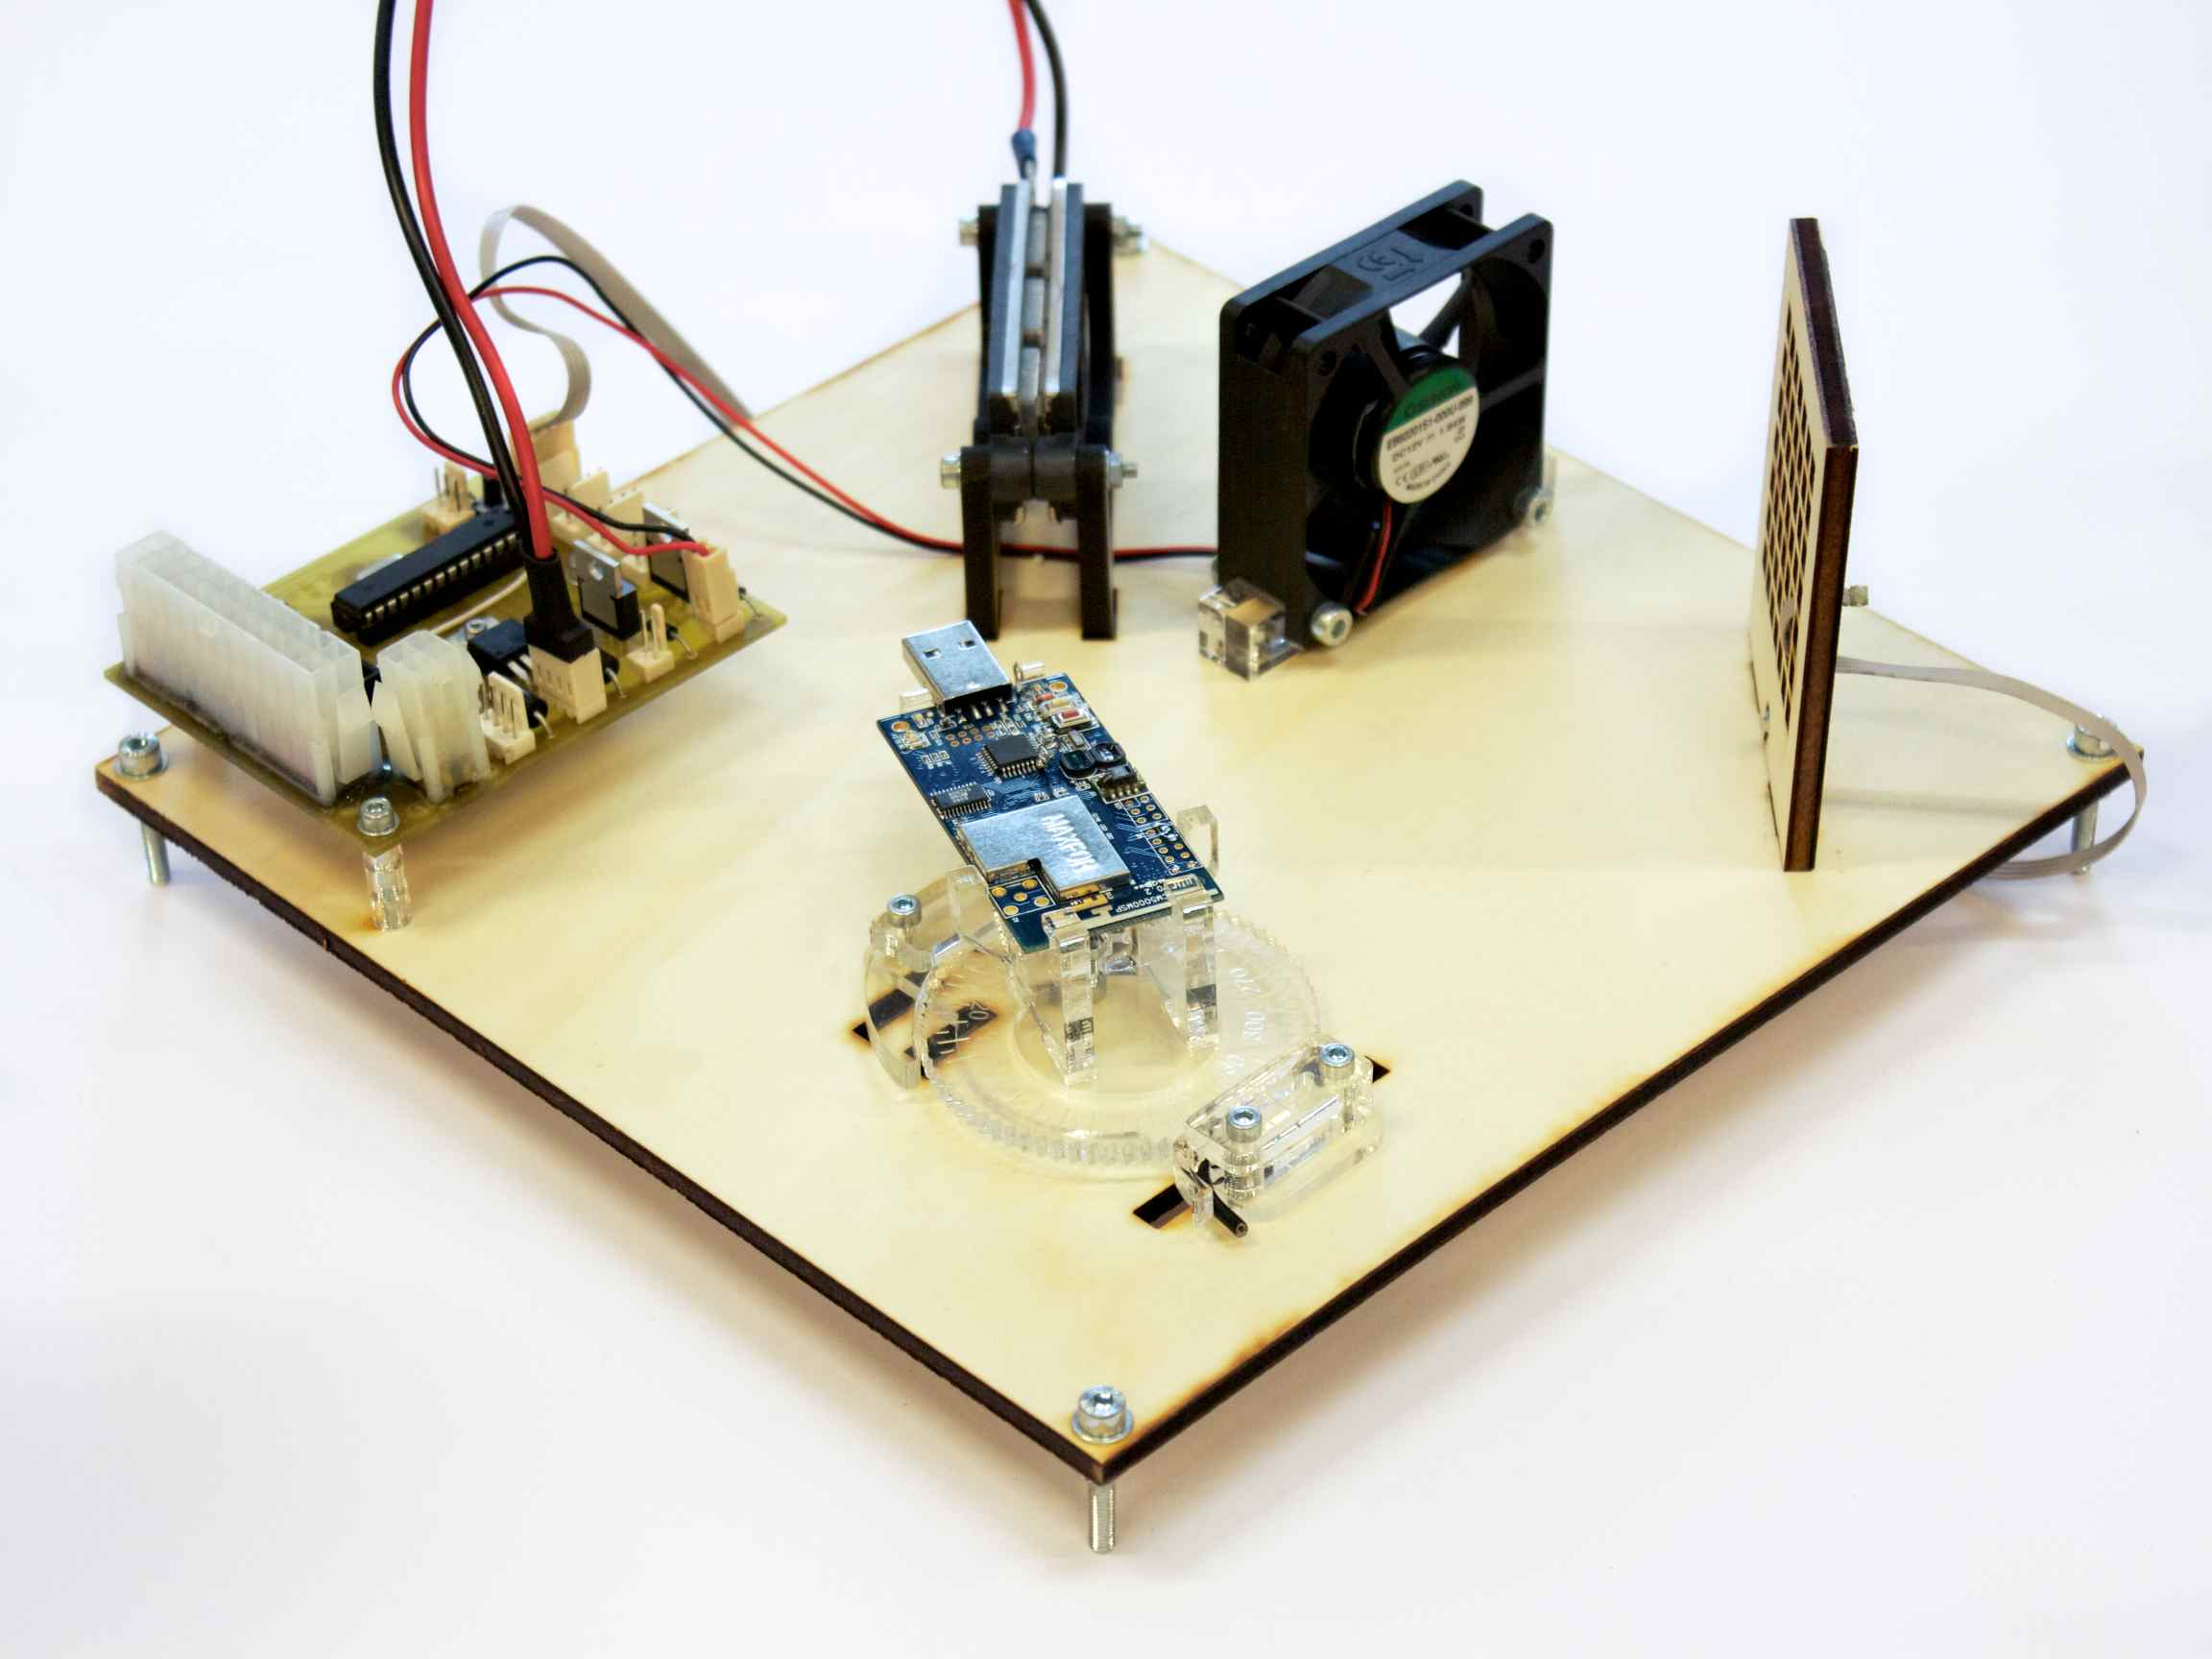
\includegraphics[width=1\columnwidth]{figures/temperature_box}
	\caption{Baseplate with temperature controller, heating element, fan and sensor mote.}
    \label{fig:box_hardware_picture}
\end{figure}


\subsection{Embedded Software}

The embedded software is written in C++ using the xpcc microcontroller framework~\cite{xpcc.io} and implemented as a set of asynchronous control tasks for input parsing and output formatting, temperature sensor evaluation, \acs{PID} loop update and duty cycle generation.
The choice of an ATmega328 as a microcontroller was deliberate to enable compatibility with the Arduino framework, which might be more familiar to developers.

Once the controller is programmed via \ac{ISP}, it will periodically send the values of all attached temperature sensors, as well as the current heating element power setting in human-readable ASCII format.
Desired temperature can be sent as an ASCII formatted integer followed by the letter `C'.
All switching frequencies were kept well below \SI{1}{\kilo\hertz} to avoid any kind of interference with the \SI{2.4}{\giga\hertz} band.


\subsection{Performance}

The heating element has enough power to heat the air inside the box up to \SI{120}{\celsius}.
This can however damage both the \ac{PS} material as well as the mote, so a hard limit of \SI{90}{\celsius} is imposed during experiments.

As seen in Figure~\ref{fig:box_heating_cooling} it takes about 40 minutes to heat up to \SI{90}{\celsius} and about 2 hours to cool back down to \SI{30}{\celsius}.
The \acs{PID} loop is deliberately dampened so that no overshoot in air temperature occurs, however, since the mote temperature naturally lags behind, a slight overshoot in air temperature might actually help achieve desired mote temperature quicker.
However, during the experiments a more granular approach is used similar to Figure~\ref{fig:box_heating_step}.

The boxes can be retrofitted with an active piezoelectric cooling element and a fan by connecting them to the two unused \acs{MOSFET} switches on the controller and updating the software, which also allow reaching temperatures below room temperature.
Since we did not use a cooling element, we set the minimum experiment temperature at \SI{30}{\celsius} so that in a room temperature of $20-$\SI{25}{\celsius} it can still be reached within reasonable time.

\begin{figure}[t]
	\subfigure[Heating to \SI{90}{\celsius}, then cooling to \SI{30}{\celsius}.] {
    	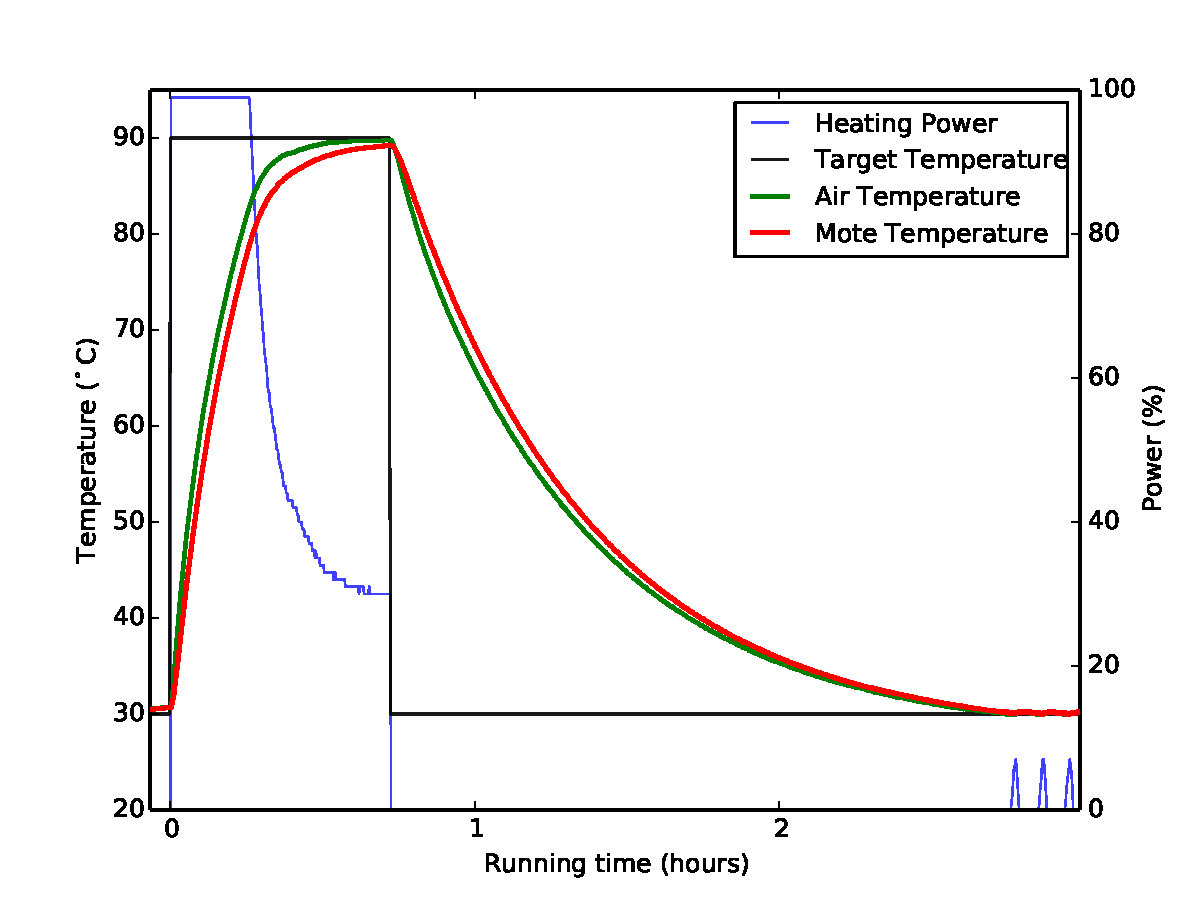
\includegraphics[width=0.475\columnwidth]{figures/box_heating_cooling}
    	\label{fig:box_heating_cooling}
    }
    \subfigure[Temperature increments of \SI{5}{\celsius}.] {
	    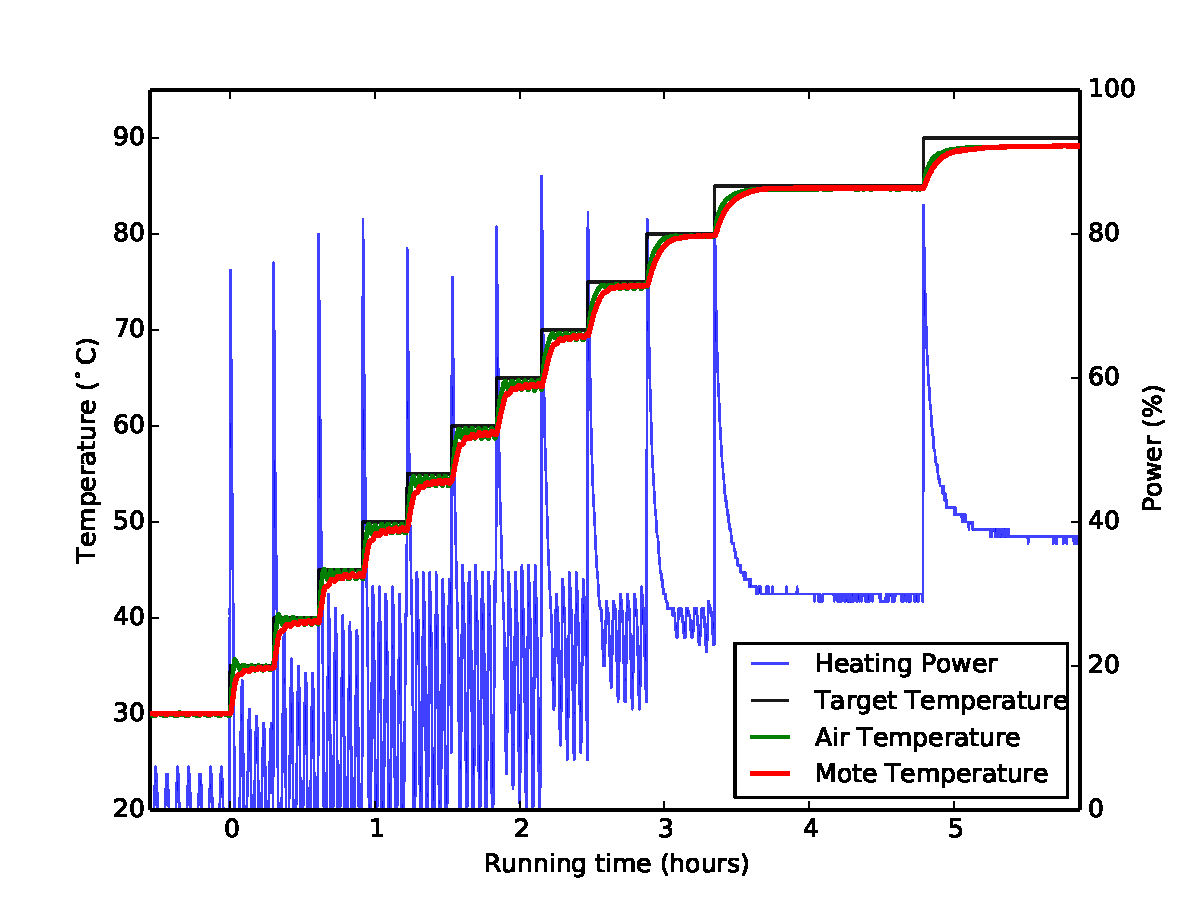
\includegraphics[width=0.475\columnwidth]{figures/box_heating_step}
	    \label{fig:box_heating_step}
	}
	\caption{Typical performance of the boxes over time. Notice the mote temperature (red line) lagging behind air temperature (green line).}
	\label{fig:box_heating_curves}
\end{figure}

Compared to TempLab by Boano~\etal~\cite{Boano2014}, which uses infrared heat lamp controlled via the wireless Z-Wave home automation protocol, our boxes require more manual assembly, do not operate wirelessly and cannot change temperature as fast.
However, our boxes also only cost one third as much (\EUR{91} versus \EUR{293}).

% \newpage
